\documentclass[12pt,a4paper,oneside]{memoir}
\usepackage[utf8]{inputenc}
\usepackage[T1]{fontenc}
\usepackage{microtype}
\usepackage[dvips]{graphicx}
\usepackage{xcolor}
\usepackage{times}
\usepackage{ragged2e}

\usepackage[
breaklinks=true,colorlinks=true,
%linkcolor=blue,urlcolor=blue,citecolor=blue,% PDF VIEW
linkcolor=black,urlcolor=black,citecolor=black,% PRINT
bookmarks=true,bookmarksopenlevel=2]{hyperref}

\usepackage{biblatex}
\addbibresource{sample.bib}

\newenvironment{acknowledgement}%       New acknowledgement environment
    {\large\bfseries\centering ACKNOWLEDGEMENT%
    \par\medskip\normalfont\normalsize}%
    {}%

\newenvironment{candidate}%       New acknowledgement environment
    {\large\bfseries\centering CANDIDATE'S DECLARATION%
    \par\medskip\normalfont\normalsize}%
    {}%


\newenvironment{certificate}%       New acknowledgement environment
    {\large\bfseries\centering CERTIFICATE%
    \par\medskip\normalfont\normalsize}%
    {}%

\newenvironment{abs}%       New acknowledgement environment
    {\large\bfseries\centering ABSTRACT%
    \par\medskip\normalfont\normalsize}%
    {}%


\usepackage{titlesec}
\newcommand*{\justifyheading}{\raggedleft}
\titleformat{\chapter}[display]
  {\normalfont\Large\bfseries\justifyheading}{\chaptertitlename\ \thechapter}
  {10pt}{\vspace{1.5ex}}
  [\vspace{1ex}\titlerule]
\titlespacing*{\chapter}{-20pt}{-5pt}{10pt}



\usepackage{geometry}
% PDF VIEW
% \geometry{total={210mm,297mm},
% left=25mm,right=25mm,%
% bindingoffset=0mm, top=25mm,bottom=25mm}
% PRINT
\geometry{total={210mm,297mm},
left=20mm,right=20mm,
bindingoffset=10mm, top=25mm,bottom=25mm}

\OnehalfSpacing
%\linespread{1.3}

%%% CHAPTER'S STYLE
%\chapterstyle{bianchi}
%\chapterstyle{ger}
%\chapterstyle{madsen}
\chapterstyle{ntglike}
%\chapterstyle{ell}
%%% STYLE OF SECTIONS, SUBSECTIONS, AND SUBSUBSECTIONS
\setsecheadstyle{\bfseries\sffamily\raggedright}
\setsubsecheadstyle{\bfseries\sffamily\raggedright}
\setsubsubsecheadstyle{\bfseries\sffamily\raggedright}


%%% STYLE OF PAGES NUMBERING
%\pagestyle{companion}\nouppercaseheads 
%\pagestyle{headings}
%\pagestyle{Ruled}
\pagestyle{plain}
\makepagestyle{plain}
\makeevenfoot{plain}{\thepage}{}{}
\makeoddfoot{plain}{}{}{\thepage}
\makeevenhead{plain}{}{}{}
\makeoddhead{plain}{}{}{}

\setsecnumdepth{subsubsection}
\maxsecnumdepth{subsubsection} % chapters, sections, and subsections are numbered
\settocdepth{subsubsection}
\maxtocdepth{subsubsection} % chapters, sections, and subsections are in the Table of Contents


%%%---%%%---%%%---%%%---%%%---%%%---%%%---%%%---%%%---%%%---%%%---%%%---%%%

\begin{document}

%%%---%%%---%%%---%%%---%%%---%%%---%%%---%%%---%%%---%%%---%%%---%%%---%%%
%   TITLEPAGE
%
%   due to variety of titlepage schemes it is probably better to make titlepage manually
%
%%%---%%%---%%%---%%%---%%%---%%%---%%%---%%%---%%%---%%%---%%%---%%%---%%%
\thispagestyle{empty}

{%%%
\sffamily
\centering
\Large

~\vspace{\fill}

{\huge 
Improved part of speech tagging model of hindi language
}

\vspace{2.5cm}

{\LARGE
Jagjit Singh
}

\vspace{3.5cm}

A thesis submitted in partial fulfillment for the\\
degree of Masters of Technology\\[1em]
in the\\[1em]
North West Institute of Engineering and Technology, Moga

\vspace{3.5cm}

Supervisor: Lakhvir Singh Garcha

\vspace{\fill}

June 2016

%%%
}%%%

%\cleardoublepage
%%%---%%%---%%%---%%%---%%%---%%%---%%%---%%%---%%%---%%%---%%%---%%%---%%%
%%%---%%%---%%%---%%%---%%%---%%%---%%%---%%%---%%%---%%%---%%%---%%%---%%%
%-----------------------------------------------------------------------------------------------------------------------------------------------------
\newpage
\begin{candidate}
\addcontentsline{toc}{chapter}{Candidate's Declaration}
%\noindent\makebox[\linewidth]{\rule{\paperwidth}{1.0pt}}
\noindent\rule{17cm}{1.0 pt} \\

\justify
I hereby certify that I am student of M.Tech (regular) of Computer Science and engineering Department and declare that I own the full responsibility for the information, results etc. provided in this thesis titled \textbf{“Improved Part of speech tagging model for hindi language”} Submitted to \textbf{North west institute of engineering and technology } for the award of \textbf{Master of Technology in Computer Science and Engineering} degree. I have taken care in all respect to honor the intellectual property right and have acknowledged the contributions of others for using them in this academic purpose. I further declare that in case of any violation of intellectual property right or copyright, I as a candidate will be fully responsible for the same. My supervisors and institute should not be held for full or partial violation of copy right if found at any stage of my degree.
\vspace{3 cm}

\noindent Place:  Moga   \hfill Jagjit Singh \\
\noindent Date: \hfill Reg.No. 
\end{candidate}
%---------------------------------------------------------------------------------------------------------------------------------------------------
\newpage
\begin{certificate}
\addcontentsline{toc}{chapter}{Certificate}
\noindent\rule{16cm}{1.0 pt} \\
\justify
This is to certify that the thesis work entitled \textbf{“Improved Part of speech tagging model for hindi language”}, submitted by Jagjit Singh, Reg. no \_ \_ \_ \_ \_ \_ to the North west institute of engineering and technology, Moga, for the partial fulfillment of the requirement of the degree of Masters of Technology in Computer Science and Engineering is a record of student’s own study under my supervision and guidance. \\

This thesis has not been submitted to any other university or institution for the award of any other degree. \\
\vspace{3 cm}

\hfill \textbf{Supervisor}\\
\vspace{0 mm}
\hfill Pr. lakhvir Singh Garcha \\
\vspace{0 mm}
\hfill Assistant Professor\\
\vspace{0 mm}
\hfill Department of Computer Science and Engg.\\
\vspace{0 mm}
\hfill NWIET, Moga\\
\vspace{2 cm}

The M.Tech Viva-Voice examination of \textbf{Jagjit Singh} has been held on  \_\_\_\_\_\_. \\

\vspace{2 cm}

\noindent \textbf{Sign. of Supervisor}   \hfill \textbf{Sign. of External} \\
\noindent  \textbf{Examiner}  \\

\vspace{2 cm} 

\noindent  \textbf{Sign. of H.O.D} 

\end{certificate}

%---------------------------------------------------------------------------------------------------------------------------------------------------

\newpage
\begin{acknowledgement}
\addcontentsline{toc}{chapter}{Acknowledgement}
\noindent\rule{17cm}{1.0 pt} \\

\justify
First of all I would like to thank Almighty God. It’s only because of the blessings of the God that I have been able to complete my thesis work successfully. I would like to thank \textbf{Pr. Lakhvir Singh Garcha} for being my advisor, and for her guidance and support throughout my research work.Also i like to thank \textbf{Dr. Mohita Garg} Head of Department for her valuable suggestions about the research work. I am deeply grateful for all the help I have received during the course of this thesis at North west institute of engineering and technology, Moga. I am also thankful to all the staff members of the CSE department  who have helped me in many ways directly or indirectly for this research work. \\


Finally I would like to thank my dear parents whose moral support and care always encouraged me to proceed.\\

\vspace{3 cm}

\hfill \textbf{Jagjit Singh}

\end{acknowledgement}
%----------------------------------------------------------------------------------------------------------------------------------------------------
\newpage
\begin{abs}
\addcontentsline{toc}{chapter}{Abstract}
\noindent\rule{16cm}{1.0 pt} \\
\justify
Part-of- Speech tagging is the way to tag every word in a text as a particular part of speech, e.g. proper verb, adverb etc. POS tagging is the first important step in the processing of NLP applications. This paper reports the improved model POS tagging for Hindi  Languages. Due to complex structural effect, the number of problems occurs when tagging the sentences written in various languages. So we, in this research try to make a model, which could improve the word sentence tagging to a gereater extent as compare to the previous models. We define 25 types of tags in the research, and details of these tag are briefly discussed in this book.
\end{abs}
%\begin{abstract}
%\addcontentsline{toc}{chapter}{Abstract}
%   abstract-text
%\end{abstract}

\newpage


\tableofcontents*

\newpage
\listoffigures
\newpage
\listoftables
\clearpage




%%%---%%%---%%%---%%%---%%%---%%%---%%%---%%%---%%%---%%%---%%%---%%%---%%%
%%%---%%%---%%%---%%%---%%%---%%%---%%%---%%%---%%%---%%%---%%%---%%%---%%%

\chapter{INTRODUCTION}

This chapter provides the introduction of NLP (natural language processing) and architecture of POS tagging process. It presents features and applications of POS taggers.  It also describes different methods of tagging.

\section{Context}

With the advancement of technology, the demand of Natural Language Processing (NLP) is also increasing and it becomes very important to find out correct information from collection of huge data only on the basis of queries and keywords. Sometimes user tries to search data with help of query and get unimportant or irrelevant data instead of correct data. Due to complex structural effect, this problem occurs mostly with Indian languages as compared to others. To avoid this problem, POS tagging is the best application of NLP that assigns exact part of speech to each word of a text (Mohnot, K, 2014). It is the process of marking up a word in a corpus as corresponding to a particular part of speech use its definition, as well as its relation. POS tags are also known as word classes, morphological classes, or lexical tags to choose correct grammatical tag for word on the basis of linguistic feature. 

There are a number of approaches to implement part of speech tagger, i.e. Rule Based approach, Statistical approach and Hybrid approach. Rule-based tagger use linguistic rules to assign the correct tags to the words in the sentence or file. Statistical Part of Speech tagger is based on the probabilities of occurrences of words for a particular tag. Hybrid based Part of Speech tagger is combination of Rule based approach and Statistical approach. Part of Speech tagging is an important application of natural language processing. It is used in several Natural Languages processing based software implementation. Accuracy of all NLP tasks like grammar checker, phrase chunker, machine translation etc. depends upon the accuracy of the Part of Speech tagger. Tagger plays an important role in speech recognition, natural language parsing and information retrieval (Mehta, D. N, 2015).

NLP (natural language processing) is the process that provides the facility of interaction between human and machine. It is a component of computer science, linguistics and artificial intelligence. It is difficult task to build NLP application because human speech is not always specific. The main objective of NLP is to develop such a system that can understand text and translate between human language and another. The work in area of Part-of-Speech (POS) tagging has begun in the early 1960s. Part of Speech tagging is an important tool for NLP. It is one of the simplest as well as statistical models for many NLP applications. POS Tagging is an initial step of information extraction, summarization, retrieval, machine translation, speech conversion.

POS tagging is the process of assigning the best grammar tag to each word of text like verb, noun, pronoun , adjective , adverb, conjunction , preposition etc. some unknown words exist in every language so it is very difficult task to assign the appropriate POS tag to each word in a sentence [3]. The mostly work that has been done for Indian languages was one of the rule based approaches and other empirical based POS tagging Approach. But the fact was that rule-based approach requires proper language knowledge and hand written rule.  Due to morphological effect of Indian languages, researchers faced a great problem to write proper linguistic rules and many cases it was noticed that results were not good. Most of natural language processing work has been done for Hindi, Tamil, Malayalam and Marathi and several part-of-speech taggers have been applied for these languages. After this, researchers moved to stochastic based approach. However the stochastic methods requires  large corpora to be effective, but still many successful POS were developed and used in various natural language processing tasks for Indian language. 

The main issue after morphological richness of Indian Languages is Ambiguity. It is very time consuming process to assign a correct POS tag to different context words. Due to this reason, POS Tagging is becoming a challenging problem for study in the field of NLP.

The main objective of Natural Language Processing is to facilitate the interaction between human and machine. POS tagging is the process of attaching the best grammar tag like to each word of a sentence of some language. A word in a sentence can act as a verb, noun, pronoun, adjective, adverb, conjunction, preposition etc so POS is defined as the grammatical information of each word of a sentence. While assigning a POS tag it is necessary to determine the context of the word i.e. whether it is acting like a noun, adjective, verb etc. Sometime a word can act as a noun in one sentence and in another sentence it can give the sense of verb. So before selecting a POS tag for a word the exact context of the word must be clear. For Indian languages it is a difficult task to assign the correct POS tag to each word in a sentence because of some unknown words in Indian languages. The earlier work that has been done for Indian languages was based rule based approaches. But the rule-based approach needs proper language knowledge and hand written rule. Most of natural language processing work has been done for Hindi, Tamil, Malayalam and Marathi and several part-of-speech taggers have been applied for these languages. The set of tags assigned by a part of speech tagger may contain just a dozen tags so such a big tagset can arise the difficulty in the tagging process. POS tagging is helpful in various NLP tasks like Information Retrieval, Machine Translation, Information Extraction, Speech Recognition etc. For Indian languages researchers find difficulty in writing linguistic rules for rule based approaches because of morphological richness. The other main issue after morphological richness of Indian Languages is Ambiguity. It is very time consuming process to assign a POS tag to each word according to its context in sentence by hand and that is why POS Tagging is becoming a challenging problems for study in the field of NLP

\section{Tagging}
Automatic assignment of descriptors to the given tokens is called tagging. The descriptor is called tag. The tag may indicate one of the part of speech, semantic information and soon. So tagging is kind of classification. 


\section{POS Tagger}
The broad utilization of internet for making search of information is difficult due to the search systems consist container of words which causes problem in retrieval due to synonyms. There is need to accept the word boundary between what kinds of query information are submitted by humans and what kinds further result get (Tapaswi, N., \& Jain, S., 2012). So for text indexing and retrieval uses POS information. POS tagging is used as an early stage of text analysis in many applications such as subcategory acquisition, text to speech synthesis and alignment of parallel corpora. POS tagging is a necessary pre-module and building block for various NLP tasks like Machine translation, Natural language text processing and summarization, User interfaces, Multilingual and cross language information retrieval, Speech recognition, Artificial intelligence, Parsing , Expert system and so on. Parts of speech (POS) tagging are one of the most well studied problems in the field of Natural Language Processing (NLP). Different approaches have already been tried to automate the task for English and other western languages there are large numbers of POS tagger available for English language which has got satisfactory performance but cannot be applied to Marathi language. Part-of-speech tagging in Marathi language is a very complex task as Marathi is highly inflectional in nature and free word order language (Mehta, D. N., \& Desai, N. P. 2015). The process of assigning description to the given word is called Tagging. The descriptor is called tag. The tag may indicate one of the parts-of-speech like noun, pronoun, verb, adjective, adverb, preposition, conjunction, and interjection. The input (Raw Text) is tokenized and a corpus is used for detecting the corresponding part of speech of each token in the sentence. For correct POS tagging, training the tagger, corpus and a proper tagset is also important Disambiguation is the most difficult problem in tagging. The ambiguity which is identified in the tagging module is resolved using the grammar rules. 


\subsection{Architecture of POS tagger}

\begin{itemize}
  \item[$\bullet$] \textbf{Tokenization:} Tokenization is the process of separating tokens from raw text. Words are separated by white spaces or punctuation marks. The sentence is segmented by using white space because the occurrence of white space indicates the existence of a word boundary. There are various morphological problems where this approach fails. So by using this we can easily find out the tokens from the sentence. The given text is divided into tokens so that they can be used for further analysis. The tokens may be words, punctuation marks, and utterance boundaries (Bagul P. et al., 2014).

  \item[$\bullet$] \textbf{Ambiguity look-up:} This is to use lexicon and a guesser for unknown words. While lexicon provides list of word forms and their likely parts of speech, guessers analyze unknown tokens. Compiler or interpreter, lexicon and guesser make what is known as lexical analyser.

  \item[$\bullet$] \textbf{Ambiguity Resolution:} This is also called disambiguation. Disambiguation is based on information about word such as the probability of the word. Disambiguation is also based on related information or word/tag sequences. For example, the model might prefer noun analyses over verb analyses if the preceding word is a preposition or article. Disambiguation is the most difficult problem in tagging. The ambiguity which is identified in the tagging module is resolved using the Marathi grammar rules. 

  \item[$\bullet$] \textbf{WordNet:}  The main relation among words in WordNet is synonymy. WordNet is an electronic database which contains parts of speech of all the words which are stored in it. It is trained from the corpus for higher performance and efficiency (Bagul, P. et al., 2014).  WordNet is a large lexical database of English. Nouns, verbs, adjectives and adverbs are grouped into sets of cognitive synonyms (synsets), each expressing a distinct concept. Synsets are interlinked by means of conceptual-semantic and lexical relations. The majority of the WordNet’s relations connect words from the same part of speech (POS). Thus, WordNet really consists of four sub-nets, one each for nouns, verbs, adjectives and adverbs, with few cross-POS pointers. Cross-POS relations include the “morph semantic” links that hold among semantically similar words sharing a stem with the same meaning.
  \item[$\bullet$] \textbf{Corpus:} For correct POS tagging, training the tagger well is very important, which requires the use of well annotated corpora. Annotation of corpora can be done at various levels which include POS, phrase or clause level, dependency level etc. Corpus linguistics is the study of language as expressed in samples (corpora) of "real world" text. Corpus is a large collection of texts. It is a body of written or spoken material upon which a linguistic analysis is based. The plural form of corpus is corpora. Some popular corpora are British National Corpus (BNC), COBUILD/Birmingham Corpus, and IBM/Lancaster Spoken English Corpus (Bagul, P. et al., 2014). 

  \item[$\bullet$] \textbf{Tagset:} Apart from corpora, a well-chosen tagset is also important. The language tagset represents parts of speech and consist on syntactic classes. According to contextual and morphological structure, natural languages are different from each other.In the top level the following categories are identified as universal categories for all ILs and hence these are obligatory for any tagset. Some common tags: [N] Nouns [V] Verbs, [PR] Pronouns, [JJ] Adjectives, [RB] Adverbs, [PP] Postpositions, [PL] Participles, [QT] Quantifiers, [RP] Particles, [PU] Punctuations (Mahar, J. A., \& Memon, G. Q., 2010).	
\end{itemize}

\section{POS Tagging Techniques}
The POS tagger can be implemented by using either a supervised technique or an unsupervised technique. Supervised POS taggers are based on pre-tagged corpora, which are used for training to learn information about the word-tag frequencies, rule and tag set, sets etc. The performance of the models generally increases with the increase in size of these corpora. 

Unsupervised POS tagging models do not require pretagged corpora. Instead, they use those methods through which automatically tags are assigned to words. Advanced computational methods like the Baum-Welch algorithm to automatically include tag sets, transformation rules etc. Under these two categories different approaches have been used for the implementation of POS taggers such as: 

\begin{enumerate}
  \item \textbf{Rule Based Approach / Transformation Based:} The rule based POS tagging approach that uses a set of hand written rules. Rule base taggers depend on word list or lexicon or dictionary to assign appropriate tag to each word. The tagger divided into two stages. First, it search words in dictionary and second, it assigns a tag by removing disambiguity of words using linguistic features of word.	

On the basis of level rule divided as lexical rules act in a word level, each sentence splits into small words called lexeme or token And, the context sensitive rules act in a sentence level, to check the grammar for the sentence. The transformation based approach is similar to the rule based approach in the sense that it depends on a set of rules for tagging. The transformation based approaches use a pre-defined set of handcrafted rules as well as automatically induced rules that are generated during training (Bagul P. et al., 2014). 

The main drawback of rule based system is that it fails when the text is not present in lexicon. Therefore the rule based system cannot predict the appropriate tags. 

  \item \textbf{Statistical Approach / Stochastic Tagger:} A stochastic approach assign a tag to word using i frequency, probability or statistics. From the annotated training data it “selects the most likely tag for the word” and uses same information to tag that word in the unannotated text (Bagul P. et al., 2014). Stochastic tagger as a simple generalization of the stochastic taggers generally resolves the ambiguity by computing the probability of a given word (or the tag).
The drawbacks of this approach are that it can come up with sequences of tags for sentences that are not acceptable according to the grammar rules. So, it determines the best tag for a word by calculating the probability of previous tags on n value, where the value of n is set to 1, 2 or 3 are known as the Unigram, Bigram and Trigram models.
 

\begin{itemize}
  \item[$\bullet$]\textbf{Hidden Markov Model:} HMM stands for Hidden Markov Model. HMM is a generative model. The model assigns the joint probability to paired observation and label sequence. Then the parameters are trained to maximize the joint likelihood of training sets .It is advantageous as its basic theory is elegant and easy to understand. Hence it is easier to implement and analyze. It uses only positive data, so they can be easily scaled. It has few disadvantages. In order to define joint probability over observation and label sequence HMM needs to enumerate all possible observation sequence. Hence it makes various assumptions about data like Markovian assumption i.e. current label depends only on the previous label. Also it is not practical to represent multiple overlapping features and long term dependencies. Number of parameter to be evaluated is huge. So it needs a large data set for training (Bagul P. et al., 2014).

  \item[$\bullet$] \textbf{ Maximum Entropy Markov Model:} MaxEnt stands for Maximum Entropy Markov Model (MEMM). It is a conditional probabilistic sequence model. It can represent multiple features of a word and can also handle long term dependency. It is based on the principle of maximum entropy which states that the least biased model which considers all known facts is the one which maximizes entropy. Each source state has an exponential model that takes the observation feature as input and output a distribution over possible next state. Output labels are associated with states.

The large dependency problem of HMM is resolved by this model. Also, it has higher recall and precision as compared to HMM. The disadvantage of this approach is the label bias problem. The probabilities of transition from a particular state must sum to one. MEMM favors those states through which less number of transitions occurs (Mohnot K \& Singh S P, 2014).

  \item[$\bullet$] \textbf{Conditional Random Field Model:} CRF stands for Conditional Random Field. It is a type of discriminative probabilistic model. It has all the advantages of MEMMs without the label bias problem. CRFs are undirected graphical models (also know as random field) which is used to calculate the conditional probability of values on assigned output nodes given the values assigned to other assigned input nodes.
\end{itemize}

  \item \textbf{Hybrid Approach:} This approach combines the advantages of both of the above approaches namely rule based approach and stochastic approach. Words in this technique are first tagged probabilistically and then as post processing, linguistic rules are applied to tag tokens. Accuracy of taggers based on this approach generally gives good results than other techniques (Mehta, D. N, 2015).
  \item \textbf{Neural Tagger:} Neural taggers are based on neural networks which learn the parameters of POS tagger from a representative training data set. The MLP-tagger is trained with error back-propagation learning algorithm. The performance has shown better than stochastic method (Raju, S. B., 2002).

\end{enumerate}

\section{Applications of POS tagger} The POS tagger can be used as a preprocessor. Text indexing and retrieval uses POS information. Speech processing uses POS tags to decide the pronunciation. POS tagger is used for making tagged corpora. 

\section{Features for POS Tagging}
The Following features have been found to be very useful in POS tagging: \\

\textbf{Suffixes} The next word of Current token is used as feature.\\

\textbf{Prefixes} The previous word of Current token is used as feature.\\

\textbf{Context Pattern based Features} Context patterns are helpful for POS tagging. Eg. Word prefixes and suffix context patterns. \\

\textbf{Word length} Length of particular word is useful feature. \\

\textbf{Static Word Feature} The previous and next words of a particular word are used as features.\\

\textbf{Presence of Special characters} Presence Special characters surrounding the current word are used as features.\\


\section{Organization of Thesis}
The structure of the rest of the Thesis is as follows:

\textbf{Chapter 2}, presents the background of various POS tagging approaches  for various languages and it covers the detail about. It also includes literature review of study. \\

\textbf{Chapter 3}, Tells about the present work, methodology in detail. It explains the algorithm and flowchart of present study.\\


\textbf{Chapter 4}, presents the results of study and compares this with existing techniques on the basis of different output parameters.\\

\textbf{Chapter 5}, contains the conclusion and future work. In the end references are marked.\\








%===================================================================================================================================================



%==============================================================================================================================================
\chapter{LITERATURE REVIEW}
\section{Literature Review}
This chapter provides the information of POS taggers for different languges and review of various techniques used for tagging.

\subsection{A glance over Related Literature}
Initial computers were design just to do simple calculations; scientists have been
trying to endow the computer with more and more intelligence. That is to make the
digital machine, do things, which require human-like intelligence. Thus the term
Artificial Intelligence (AI) was coined in early 1950s. Gradually scientists came to
know the immense power of the device and its limitations. More and more systems
have been developed as a consequence of incremental advances in computer science.
Slowly these electronics devices have been spreading their roots in the soils of this
society. Now computer systems are available for applications of civil amenities to
medical diagnosis; home entertainment to space programs; simple calculations to
complex mathematical modeling etc.

In today’s fast placed world where every human being has to combat a race against
time – a direct interface between the spoken words and computer user will gleefully
accept the same words spontaneously typed on the computer screen with minimum
lapse of time. The phenomenon is known as speech (voice) recognition.

word tagging is an emerging technology where a speaker speaks to computer
with the microphone and computer understands the given words. Speech recognition
is a great supplement to traditional mouse and keyboard input; it will boost
productivity and provide a new option for people who have difficulty using a
keyboard.\\


\textbf{Pallavi Bagul et al:} "rule based pos tagger for Marathi language."proposed a rule based pos tagger for Marathi language. The input sentence sent to tokenized function, the one which tokenizes the string into tokens and then comparing tokens with the Word Net. Tagging module assigned a tag to tokenized word and search for ambiguous word and pronoun. The ambiguous words were those words which can act as a noun and adjective in certain context, or act as an adjective and adverb in certain context. Then their ambiguity is resolved using Marathi grammar rules. Author used a corpus which is based on tourism domain called annotated corpus and 3 grammar rules are used for the experiment to resolve ambiguous word which acts a noun and adjective in certain context, or act as an adjective and adverb in certain context. 
\\

\textbf{H.B. Patil et.al:} "a Partof-Speech Tagger for Marathi Language using Limited Training Corpora" is also a rule based technique. Here sentence taken as an input generated tokens. Once token generated apply the stemming process to remove all possible affix and reduce the word to stem. SRR used to convert stem word to root word. They developed 25 SRR rule. The root-words that are identified are then given to morphological analyzer. The morphological analysis is carried out by dictionary lookup and morpheme analysis rules. Disambiguation is removed by the use of rule-base model or Hidden Markov Model. Based on the corpus they have identified 11 disambiguation rules that are used to remove the ambiguity. Stemming process removes all possible affixes, it change the meaning of stem word like (Anischit-Nischit).The size of the corpus is increased then more Rules can be discovered which will help to reduce the error rate.\\

\textbf{Jyoti Singh Nisheeth \& Joshi Iti:} "Development of Marathi Part of Speech Tagger Using Statistical Approach"  They used statistical tagger using Unigram, Bigram, Trigram and HMM Methods. To achieve higher accuracy they use set of Hand coded rules, it include frequency and probability. They train and test their model by calculating frequency and probability of words of given corpus. In unigram technique find out how many time each word occur in corpus and assign each word to most common tag. Bigram tagger makes tag suggestion based on preceding tag i.e. it take two tags previous and current tag. In Trigram provides the transition between the tags and helps to capture the context of the sentence. The probability of a sequence is just the product of conditional probabilities of its trigrams. Basic idea of HMM is assigns the best tag to a word by calculating the forward and backward probabilities of tags along with the sequence provided as an input. Powerful feature of HMM is context description. The POS taggers described here is very simple and efficient for automatic tagging, but it is difficult for Marathi as it is morphological rich language. In this paper [15],

Nidhi Mishra \& Amit Mishra proposed Part of Speech Tagging for Hindi Corpus. The system scans the Hindi (Unicode) corpus and then extracts the Sentences and words from the given Hindi corpus. Finally Display the tag of each Hindi word like noun tag, adjective tag, number tag, verb tag etc. and search tag pattern from database. The proposed model for Hindi language is apprehensible, but need to training data to increase accuracy. The efficiency of system judge on the basis of parameter of used need. \\

\textbf{ Namrata Tapaswi \& Suresh Jain:} "a Treebank Based Deep Grammar Acquisition and Part-Of-Speech Tagging for Sanskrit Sentences" In the Sanskrit morphology meaning of the word is remain same. When affixes are added to the stem, words are differentiated at data base level directly. The input is one sentence per line, split the sentence in to words called lexeme. Read each word to find longest suffix, and eliminated the suffix until the word length is 2. Apply the lexical rules and assign the tag. Remove the disambiguity using context sensitive rules. For experimental result Author taken set of 100 words and manually evaluated, The system gives 90\% correct tags for each word. The evaluation was done in two stages. Firstly by applying the lexical rules and secondly, after applying the context sensitive rule. The POS taggers described here is very efficient for Sanskrit but it is difficult for Marathi as affix is attached to root word so the meaning of word get change.\\

\textbf{Ghulam Qadir menon:} in his paper "Rule Based Part of Speech Tagging of Sindhi Language" Take input text, and generate token. Once token generated search and compare selected word from lexicon (SWL) .If word is found one or more times, then store associated tag and if not found add that word into lexicon by generating linguistic rule for new word. The tagset contains 67 tags. A lexicon named SWL is developed having entries of 26366 words. Author also found the frequency for tag. For this purpose, set of 186 disambiguation rules are used for SPOS tagging system. The contextual information is used for rule-based approach and manually assigns a part of speech tag to a word. Accuracy of 96.28\% was achieved from SPOS. When more words will be tagged and rules will be added then accuracy will be increased.\\


\textbf{Kamal Sarkar, Vivekananda Gayen:}  "A Practical Part-of-Speech Tagger for Bengali" The system has two major phases: training phase and testing phase. In the training phase, the system is trained on a handful of POS tagged Bengali sentences by computing tag transition probabilities and word likelihoods or observation probabilities. In the testing phase, untagged Bengali sentences are submitted to the system for tagging. Viterbi algorithm is used for finding the most likely tag sequence for each sentence in the input document. Author implemented a supervised Bengali trigram POS Tagger from the scratch using a statistical machine learning technique that uses the second order Hidden Markov Model (HMM).The performance of the POS tagger can be improved by introducing more accurate method for unknown word handling.\\


\textbf{Antony P J and Dr. Soman:} "a survey on developments of different POS tagger systems as well as POS tagsets for Indian languages" the existing approaches that have been used to develop POS tagger tools . They concluded that almost all existing Indian language POS tagging systems are based on statistical and hybrid approach. 

This Paper specifies A CRF (Conditional Random Fields) based part of speech tagger and chunker for Hindi had been used by Aggarwal Himashu and Amni Anirudh. After evaluation they found that the strength of Conditional Random Fields can be seen on large training data and CRF performs better for chunking rather than for POS tagging with the training on same sized data. With training on 21000 words with the best feature set, the CRF based POS tagger is 82.67\% accurate, while the chunker performs at 90.89\% when evaluated with evaluation script from conll 2000.\\

\textbf{Navneet Garg et. al.:} used Rule Based Hindi Part of Speech Tagger for Hindi. The System is evaluated over a corpus of 26,149 words with 30 different standard part of speech tags for Hindi. The evaluation of the system is done on the different domains of Hindi Corpus. These domains include news, essay, and short storie and system achieved the accuracy of 87.55\%.\\

\textbf{Brills et. al.:}specfies A Comparison of Unigram, Bigram, HMM and Brill's POS Tagging Approaches for some South Asian Languages has been done by Fahim Muhammad Hasan compared the performance of n-grams, HMM or transformation based POS Taggers on three South Asian Languages, Bangla, Hindi and Telegu. And we found that the HMM based tagger might perform better for English, but for South Asian languages, using corpora of different sizes, the transformation based Brills approach performs significantly better than any other approach when using a 26-tags tagset and pre-annotated training corpora consisting of a maximum of 25426, 26148 and 27511 tokens for Bangla, Hindi and Telegu respectively.\\

\textbf{Manjit Kaur et. al:} introduced an improving Punjabi Part of Speech Tagger by Using Reduced Tag Set. They Effort to improve the accuracy of HMM based Punjabi POS tagger has been done by reducing the tagset. The tagset has been reduced from more than 630 tags to 36 tags. We observed a significant improvement in the accuracy of tagging. Their proposed tagger shows an accuracy of 92-95\% whereas the existing HMM based POS tagger was reported to give an accuracy of 85-87\%.\\

\textbf{Nisheeth Joshi:} described efforts to build a Hidden Markov Model based Part of Speech Tagger. They used IL POS tag set for the development of tagger. HMM based statistical technique was used to train POS tagger for Hindi. They disambiguated correct word-tag combinations using the contextual information was available in the text and attained the accuracy of 92.13\% on test data.\\

\textbf{N. Garg et al.:} in their paper "Rule Based Part-of-Speech Tagger for Hindi language" Their System is tested over dataset of 26,149 words with 30 different POS tags for Hindi. They have evaluated their system on the different domain of Hindi Corpus including news, essay, and short stories. The system achieved the accuracy of 87.55\%.The system mainly works in two steps- firstly the input words are found in the database; if it is present then it is tagged. Secondly if it is not present then various rules are applied. If a sentence consists of 12 words out of which 8 words are unknown, then system fails to tag them. It is hard to decide which rules should be handled first because word tagging resolution is based on neighbor’s word and hence it fails.

\textbf{M. Shrivastava and P. Bhattacharyya} present a paper in which they have presented a simple Hidden markov model based POS tagger. As a pre-processor they have employed longest suffix matching stemmer and claim to achieve accuracy of 93.12\%. The core idea of their approach is to “explode” the input in order to increase the length of the input and to reduce the number of unique types they encountered at the time of learning. This orderly increases the probability score of the correct choice while simultaneously decreasing the ambiguity of the choices at each stage.
In 2006, H. Agrawal and A. Mani have presented paper on “Part of Speech Tagging and Chunking with Conditional Random Fields” for Hindi. In which training is performed using a morph analyzer and CRF++ to provide extra information like root word and possible Part of speech tags for training. With training on 21000 words and best feature set, they have claimed to have achieved 82.67\% accuracy.\\

\textbf{N. Joshi, H. Darbari and I. Mathur} They have used 15,200 sentences (3, 58,288 words) from tourism domain to train the system. They have used two special tags and to denote starting and ending of the sentence which was added to all the sentences of the training corpus. The accuracy of 92.13\% on test data was attained. Another Part of speech tagger by A. Ekbal, S. Mondal, and S. Bandyopadhyay Has been developed. Their tagger had been at the beginning trained on a Bengali training set of 20396 tokens. Then tested on the Bengali development test set consisting of 5022 tokens and demonstrated 90.9\% accuracy. After that their POS tagger is trained on the Hindi training set consisting of 21470 tokens and Telegu training sets consisting of 21415 tokens later. The POS tagger had been tested with Hindi and Telegu development sets, consisting of 5681 and 6098 tokens and it had demonstrated 82.05\% and 63.93\% accuracies respectively.
 
\textbf{S. Singh et al.} have developed a methodology of POS tagging which the languages having lack of corpora can make use of. Their methodology makes use of locally annotated relatively small-sized corpora of around 15,562 words, fully comprehensive morphological analysis supported by high coverage terminology and a decision tree based learning algorithm. The performance evaluation of their system was done with 4-fold cross validation on the dataset of news domain and they claim to have 93.45\% accuracy. \\

\textbf{Sandipan Dandapat et al.} presented a paper and described about a model that uses composition of supervised and unsupervised learning techniques using a Hidden Markov Model. They have made use of small tagged corpus and also large untagged corpus. They also make use of Morphological Analyzer that takes a word as input and gives all possible POS tags for the word. They took 1003 words from CIIL corpus and tagged it manually. They have obtained an overall accuracy of 95\%.\\
 
\textbf{Asif Ekbal et al.} made the tagger for Bengali using Maximum Entropy, which makes use of the different circumstantial information of the words with the variety of features that are helpful in predicting the various Part of speech classes [27]. Their tagger has been trained with a training corpus of 72, 341 word forms and it uses a tag set of 26 different POS tags, defined for the Indian languages. Tagger has demonstrated an accuracy of 88.2\% for a test set of 20K word forms.\\
 
\textbf{S. Dandapat, and S. Sarkar} on Bengali that makes use contextual information of words. They have used a structural or morphological analyzer to make better tagging accuracy of the tagger. Further, they have made use of semi-supervised learning by increasing the small labeled training dataset provided with a larger unlabeled training dataset (1,00,000 words). The tagger had an accuracy of about 89\% on the test data provided. The supervised model parameters are estimated from the annotated training data including 3085 sentences. Hidden Markov Model learned through supervised training is treated as the basic model for unsupervised learning. The model parameters are than reestimated using the Baum-Welch algorithm by training provided over a fixed set of 11,000 untagged sentences taken from CIIL (Consortium in Indian Languages) corpus. \\

\textbf{A. Ekbal et al.} have developed a POS Tagger using Conditional Random Field. They have used tag set of 26 POS tags, which are defined for the Indian languages. The POS tagger they developed has been trained and tested with the 72,341words and 20k word forms, respectively. Their experimental results show that the CRF based tagger achieves accuracy of 90.3\%.\\

\textbf{J. Singh et al.} have developed POS tagger for Marathi. They have used Trigram Method using statistical approach. The concept mainly used here is to explore the most likely POS tag for a current word based on given knowledge of previous two tags by calculating probabilities to determine which is the best sequence of tag . For testing the performance of the system, they have developed a test corpus of 2000 sentences. They claim to have got an accuracy of 91.63\%.\\
 
\textbf{H.B.Patil et al:} In this approach they have demonstrated Part-of-Speech tagger for Marathi Language which is based on rules [32]. The hand–constructed rules are learnt from corpus and some manual additions after studying the grammar of Marathi language were added. They have tried to disambiguate tagging by analyzing the grammatical feature of the current word, its antecedent word, its succeeding word, etc. After testing their tagger, they claimed to have an accuracy of about 78.82\% on three different types of data sets. P. Bagul, A. Mishra et al. Presented a paper on “Rule based POS tagger for Marathi Text”. They describe their system as the one which tokenizes the sentences into tokens and then comparing tokens with the WordNet to assign their particular tags. They had resolved the ambiguity of the words using Marathi grammar rules.\\

\textbf{K. R. Singha et al.} have presented a paper of an attempt to develop a lexicon based POS Tagger for Manipuri. They have applied a set of hand written language specific rules of Manipuri language. In this paper they have designed a 3- tier tag set for Manipuri. This tag set consists of 97 tags including generic attributes and language specific attribute values. \\

\textbf{B.S. Purkayastha et al.} has been developed for Manipuri using stochastic approach namely Hidden Markov Model. Manipuri rule-based tagger gives tagged output that is used as corpus for training. In order to measure performance of tagger they have used manually annotated test set data that consist of 97 category of Manipuri language. They had claimed to have achieved the accuracy of 92\%.\\

\textbf{Shambhavi.B.R et al.} has developed POS Tagger for Kannada language. In this POS tagging task of Kannada language they have chosen Second order Hidden Markov Model and Conditional Random Fields. Their training data consists of 51,269 tokens and test data set incorporate around 2932 tokens. Both data set are taken from EMILLE corpus. Corpus was partitioned into 95\% for training and 5\% for testing. Their experimental result shows the accuracy of the tools which is based on HMM is 79.9\% and CRF is 84.58\%.\\ 

\textbf{P.J Antony and Soman.K.P.} They have developed their own tag set which consist of 30 tags and developed part of speech Tagger using a machine learning algorithm namely Support Vector Machine for Kannada Language. A corpus was collected from Kannada news papers and books, and it is manually morphologically analyzed and tagged using their developed tag set. After the performance of the system is evaluated they found that more efficient and accurate results were obtained as compared with preceding methods for Kannada POS tagging.\\
 
\textbf{T.N. Vikram and Shalini R.} have also presented their work on Kannada Prototype morphological analyzer for south Indian language Kannada has been presented in this paper. The analyzer can simultaneously work as stemmer, spell checker and POS tagger and hence it is very efficient tool.
A Sinhala language based Part of Speech (POS) Tagger using lexical semantics and HMM has been presented by A. Jayaweera and N.G.J Dias. They have used a statistical based approach, in which the tag identification process is done by calculating the probability of tag sequence and the probability of word-likelihood from the given dataset, where the language specific knowledge is axiomatically extracted from the annotated dataset. In this research they used the Beta version of the UCSC Corpus which contains around 6,50, 000 words and from which definite words are 70000, For known words they claim to have an accuracy of more than 90\%. \\ 

\textbf{Sondi et al.} POS Tagging and chunking using CRF and Transformation Based Learning for Telugu has been described. They showed the use of Conditional Random Fields with the help of morphological information and the transformation rules in POS tagging and Chunking. How to train CRFs to achieve good accuracy over other machine learning method is shown. They have also shown how improved training Methods based on the morphological information, contextual and the lexical rules were difficult in achieving good results. They claimed to achieve an accuracy of about 77.37\% for Telugu, 78.66\% for Hindi, and 76.08\% for Bengali using CRF and TBL based POS tagger.\\





%====================================================================================================================================================


\chapter{PRESENT WORK}
\section{Motivation}
Speech is the most common mode of communication among human beings. Speech
offers a new way of interfacing with a computer that lends itself very well to solving
the problems of field-based computing. It's natural and intuitive. 

Before we take a look at what this technology is all about and how it works, we
should make a note of the fast pace at which interactive speech technologies have
been coming into the market of late. Whenever a person has to use the PC for typing a
document on any word processing software, he/she has to slog hard and spend his
valuable time in the dull and boring job of typing the document. Time is wasted,
firstly because the typing speed does not match the speed with which a person can
think, speak or hear.

In today’s fast paced
world where every human being has to combat a race against time a direct interface
between the spoken word and Pc users will gleefully accept the same words
spontaneously typed on the PC screen with minimum lapse of time. These
technologies are getting easier to work with too. In the future, speech will definitely
be the standard input mode that most of us will replace the traditional keyboard and
mouse as the standard input device [19].

The 1990s saw the first commercialization of spoken language understanding
systems. Computers can now understand and react to humans speaking in a natural
manner in ordinary languages within a limited domain. Basic and applied research in
signal processing, computational linguistics and artificial intelligence have been
combined to open up new possibilities in human-computer interfaces [21].

So all this benifits motivates me to produce a dictation system for our motheer tongue "Punjabi" language. People from different social and economic backgrounds speak with different different dialects.Computers can now understand and react to humans speaking in a natural
manner in ordinary languages within a limited domain. Basic and applied research in
signal processing, computational linguistics and artificial intelligence have been
combined to open up new possibilities in human-computer interfaces.

\newpage

\section{System Framework}

\begin{figure}[h]
    \centering
    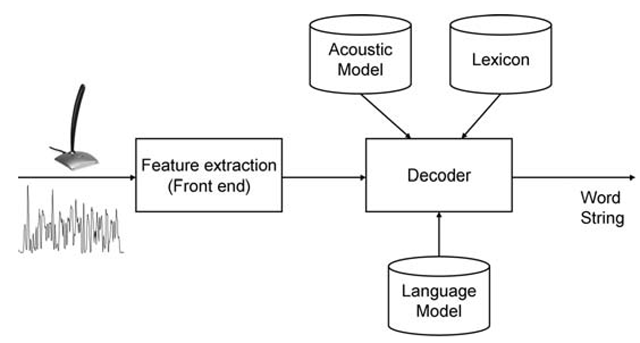
\includegraphics[scale=0.5]{tmp725d99_thumb}
%    \caption{Sphinx Architecture}
%    \label{fig:mesh1}
\end{figure}


\begin{figure}[h]
    \centering
    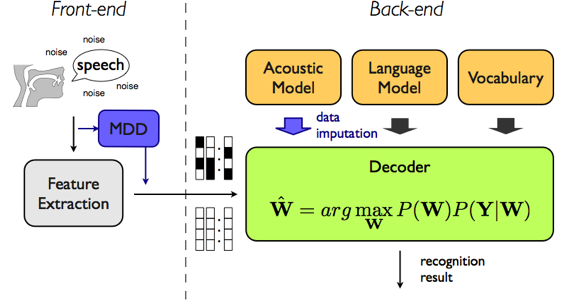
\includegraphics[scale=0.5]{mdt_recognizer}
    \caption{System Framework}
%    \label{fig:mesh1}
\end{figure}

%=====================================================================================================================================================
\chapter{EXPERIMENTAL RESULTS AND ANALYSIS}
\section{Platform}
\subsection{Operating System is Ubuntu 14.04}
Ubuntu is a Debian-based Linux operating system, with Unity as its default desktop environment. It is based on free software and named after the Southern African philosophy of ubuntu (literally, "human-ness"), which often is translated as "humanity towards others" or "the belief in a universal bond of sharing that connects all humanity".

Development of Ubuntu is led by UK-based Canonical Ltd. a company owned by South African entrepreneur Mark Shuttleworth. Canonical generates revenue through the sale of technical support and other services related to Ubuntu. The Ubuntu project is publicly committed to the principles of open-source software development; people are encouraged to use free software, study how it works, improve upon it, and distribute it [24].
\subsection{Bison}
Bison is a general-purpose parser generator that converts an annotated context-free grammar into a deterministic LR or generalized LR (GLR) parser employing LALR(1) parser tables. As an experimental feature, Bison can also generate IELR(1) or canonical LR(1) parser tables. Once you are proficient with Bison, you can use it to develop a wide range of language parsers, from those used in simple desk calculators to complex programming languages.

Bison is upward compatible with Yacc: all properly-written Yacc grammars ought to work with Bison with no change. Anyone familiar with Yacc should be able to use Bison with little trouble. You need to be fluent in C or C++ programming in order to use Bison. Java is also supported as an experimental feature [25].
\subsection{Swig}
To help build extension modules, SWIG is packaged with a library of support files that you can include in your own interfaces. These files often define new SWIG directives or provide utility functions that can be used to access parts of the standard C and C++ libraries. This chapter provides a reference to the current set of supported library files [26].
\subsection{Gstreamer} 
GStreamer is a pipeline-based multimedia framework written in the C programming language with the type system based on GObject.

GStreamer allows a programmer to create a variety of media-handling components, including simple audio playback, audio and video playback, recording, streaming and editing. The pipeline design serves as a base to create many types of multimedia applications such as video editors, streaming media broadcasters and media players.

It is designed to work on a variety of operating systems, e.g. Linux kernel-based operating systems, the BSDs, OpenSolaris, Android, OS X, iOS, Windows, OS/400.

GStreamer is free and open-source software subject to the terms of the GNU Lesser General Public License (LGPL) and is being hosted at freedesktop.org [27].
 	
GStreamer has been ported to a wide range of operating systems, processors and compilers. These include but are not limited to Linux on x86, PPC and ARM using GCC. Solaris on x86 and SPARC using both GCC and Forte, MacOSX, Microsoft Windows using MS Visual Developer, IBM OS/400 and Symbian OS.

GStreamer can bridge to other multimedia frameworks in order to reuse existing components (e.g. codecs) and use platform input/output mechanism [28].

\subsection{Gcc}
GCC was originally written as the compiler for the GNU operating system. The GNU system was developed to be 100 percent free software, free in the sense that it respects the user's freedom.

We strive to provide regular, high quality releases, which we want to work well on a variety of native and cross targets (including GNU/Linux), and encourage everyone to contribute changes or help testing GCC. Our sources are readily and freely available via SVN and weekly snapshots [27].

\subsection{Automake} 
Automake is a tool for automatically generating Makefile.in files compliant with the GNU Coding Standards. Automake requires the use of Autoconf [31]. The Automake manual can be read on-line or downloaded in PDF format; also, more formats are offered for download or on-line reading. If you have installed Automake on your system, you may also find more information about it by looking at your local documentation; for example you might use info automake at the shell prompt [27]. 
 
\subsection{Autoconf}
Autoconf is an extensible package of M4 macros that produce shell scripts to automatically configure software source code packages. These scripts can adapt the packages to many kinds of UNIX-like systems without manual user intervention. Autoconf creates a configuration script for a package from a template file that lists the operating system features that the package can use, in the form of M4 macro calls [28].

\subsection{Libtool}
 GNU libtool is a generic library support script. Libtool hides the complexity of using shared libraries behind a consistent, portable interface.

To use libtool, add the new generic library building commands to your Makefile, Makefile.in, or Makefile.am [28].




\section{Speech Recognition Engine}
\subsection{Library}
\subsubsection{Sphinxbase}
This package contains the basic libraries shared by the CMU Sphinx
trainer and all the Sphinx decoders (Sphinx-II, Sphinx-III, and
PocketSphinx), as well as some common utilities for manipulating
acoustic feature and audio files.

Sphinxbase uses the standard unix autogen system, and there's a script
included, 'build for iphone.sh' that will setup configure to create
binaries that are XCode friendly.

 ./autogen.sh

\subsubsection{Python-dev}
Header files, a static library and development tools for building
 Python modules, extending the Python interpreter or embedding Python
 in applications [20].

\subsection{Decoder}
\subsubsection{PocketSphinx}
 PocketSphinx is CMU’s fastest speech recognition system. It’s a library written in pure C which is optimal for development of your C applications as well as for development of language bindings. At real time speed it’s the most accurate engine, and therefore it is a good choice for live applications.

It's good for desktop applications, command and control and dictation where fast response and low resource consumption are the goals.

Also it includes support for embedded devices with fixed-point ariphmetics and is successfully used on IPhone, Nokia devices and on Windows Mobile. You can find further documentation about PocketSphinx in the release documentation, or at the online  documentation [29]. 

\subsubsection{Sphinx-4}
Sphinx-4 is a state-of-the-art speech recognition system written entirely in the Java™ programming language. It's best for implementation of complex server or cloud-based system with deep interaction with NLP modules, web services and cloud computing [29].

\subsection{Trainer}
\subsubsection{SphinxTrain}
 New openfst-based G2P trainer and decoder, supported by Sphinx4 too. It includes Parallel feature extraction.  Package can be installed now just like any application. Single 'sphinxtrain' command to access all training process. Increased reuse of sphinxbase functions [30].

\subsection{Experimental Setup}

\begin{enumerate}
  \item Installation of OS(operating system) i.e Ubuntu
  \item Install Bison 
  \item Install Swig
  \item Install Python-dev
  \item Install Automake 
  \item Install Autoconf
  \item Install Libtool
  \item Download Sphinxbase-5prealpha and compile it and then install from the source
  \item Download PocketSphinx-5prealpha and compile it and then install from the source
  \item Install Gstreamer  
  \item Download SphinxTrain-5prealpha and compile it and then install from the source	
\end{enumerate}

\section{Dictation System Setup}
Dictation system setup includes the making of Acoustic model and Language model for the Punjabi language. Also the use of CMULTK and testing on the PocketSphinx decoder.

\subsection{Testing the Decoder}
Before proceeding further it is important to check the existing decoder for the existing language model, so i test it with the exixting English model.
So i used Ubuntu terminal for this purpose.\\ 

\begin{figure}[h]
    \centering
    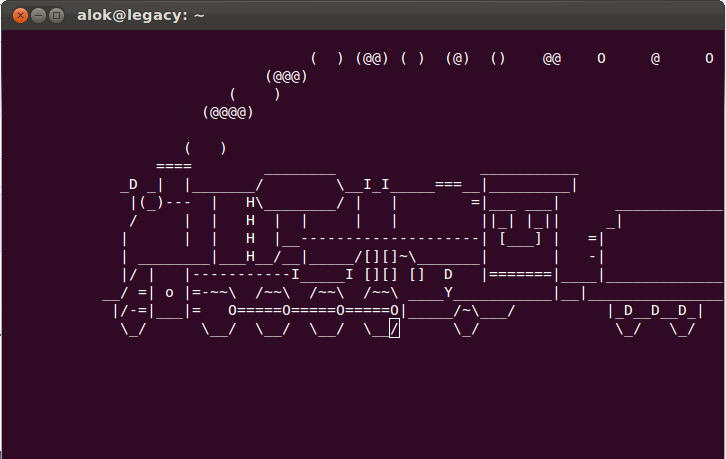
\includegraphics[scale=0.55]{networknuts-linux-fun}
    \caption{Ubuntu Terminal}
%    \label{fig:mesh1}
\end{figure}

The sphinxbase will be installed in /usr/local/ folder by default. Not every system loads libraries from this folder automatically. To load them you need to configure the path to look for shared libaries. It can be done either in the file /etc/ld.so.conf or with exporting environment variables:
\\
\textit{export LD\_LIBRARY\_PATH=/usr/local/lib} \\
\textit{export PKG\_CONFIG\_PATH=/usr/local/lib/pkgconfig}


To test installation, run 'pocketsphinx\_continuous -inmic yes' and check that it recognizes words you are saying to the microphone. 

\begin{figure}[h]
    \centering
    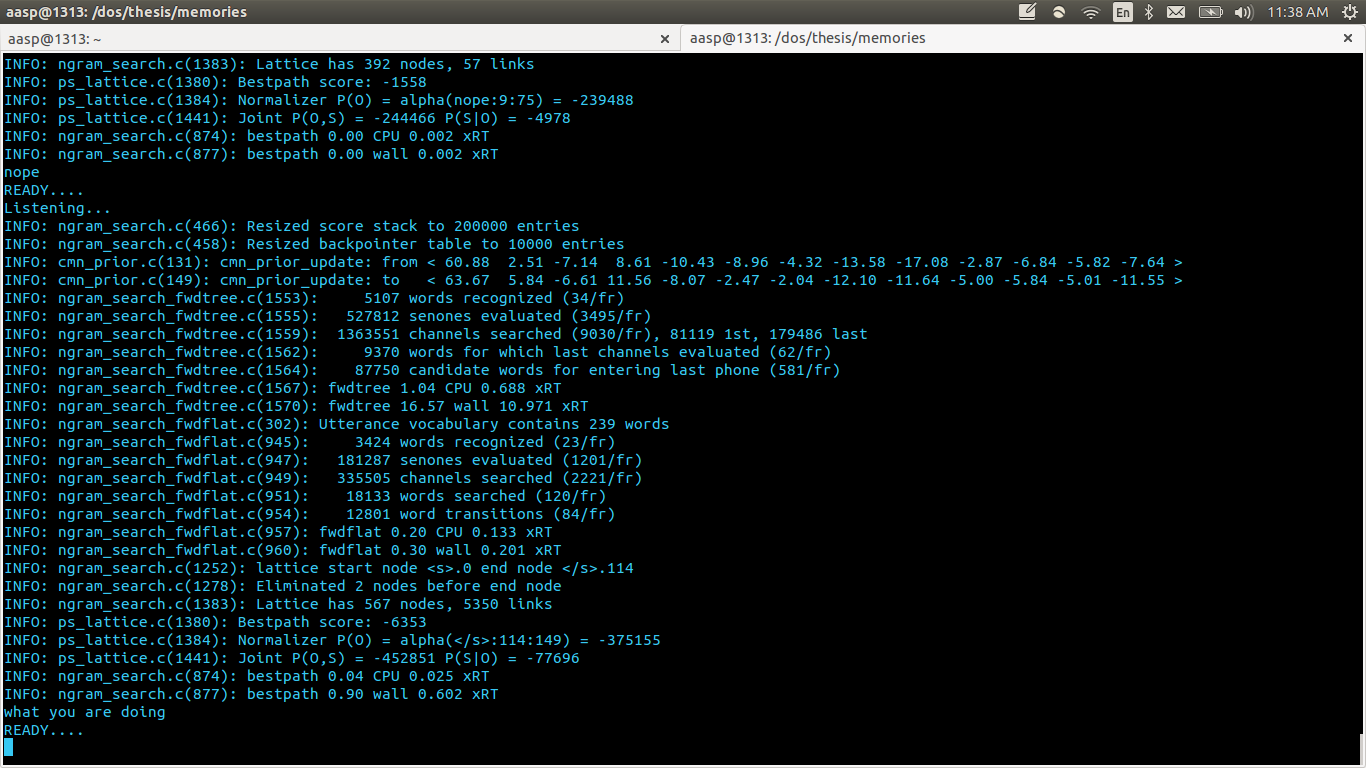
\includegraphics[scale=0.3]{Screenshot1}
    \caption{PocketSphinx Test}
%    \label{fig:mesh1}
\end{figure}

\subsection{Building Language Model}


There are two types of models that describe language - grammars and statistical language models. Grammars describe very simple types of languages for command and control, and they are usually written by hand or generated automatically with scripting code. Grammars usually do not have probabilities for word sequences, but some elements might be weighed. Grammars could be created with JSGF format and usually have extension like .gram or .jsgf.\\\\
Statistical language models describe more complex language. They contain probabilities of the words and word combinations. There are many ways to build the statistical language models. When your data set is large, there is sense to use CMU language modeling toolkit. When a model is small, you can use an online quick web service. When you need specific options or you just want to use your favorite toolkit which builds ARPA models, you can use it.
\\\\
Language model can be stored and loaded in two different format - text ARPA format and binary DMP format. ARPA format takes more space but it is possible to edit it. ARPA files have .lm extension. DMP format takes significantly less space and faster to load. DMP files have .lm.dmp extension. It is also possible to convert between formats.

\subsubsection{Text Preparation}
First of all you need to cleanup text. Expand abbreviations, convert numbers to words, clean non-word items. Language modeling for Mandarin is largely the same as in English, with one addditional consideration, which is that the input text must be word segmented. A segmentation tool and associated word list is provided to accomplish this. 
\subsubsection{ARPA Model Training}
The process for creating a language model is as follows:
\begin{enumerate}
  \item  Prepare a reference text that will be used to generate the language model. The language model toolkit expects its input to be in the form of normalized text files, with utterances delimited by <s> and </s> tags. A number of input filters are available for specific corpora such as Switchboard, ISL and NIST meetings, and HUB5 transcripts. The result should be the set of sentences that are bounded by the start and end sentence markers: <s> and </s>. Here's an example: 

\begin{figure}[h]
    \centering
    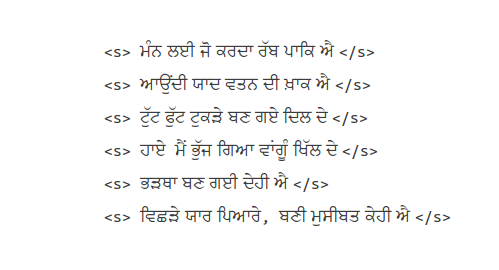
\includegraphics[scale=1.0]{Screenshot2}
    \caption{Text Prepration}
%    \label{fig:mesh1}
\end{figure}

More data will generate better language models. 

  \item  Generate the vocabulary file. This is a list of all the words in the file:

	\textit{text2wfreq < weather.txt | wfreq2vocab > weather.tmp.vocab} 
  \item Edit the vocabulary file to remove words (numbers, misspellings, names).
  \item Remove sentences from your input transcript that contain words that are not in your vocabulary file.
  \item Generate the arpa format language model with the commands:

	 \textit{text2idngram -vocab weather.vocab -idngram weather.idngram < weather.closed.txt \\
	 idngram2lm -vocab\_type 0 -idngram weather.idngram -vocab \ \\
     	 weather.vocab -arpa weather.lm}
  \item Generate the CMU binary form (DMP) 

	\textit{sphinx\_lm\_convert -i weather.lm -o weather.lm.DMP}
\end{enumerate}

\subsubsection{Using Language Model with PocketSphinx}

\textit{pocketsphinx\_continuous} can be run from the command-line to recognize speech. Assuming it is installed under \textit{/usr/local}, and your language model and dictionary are called \textit{.dic} and \textit{.lm} and placed in the current folder, try running the following command: 

\textit{pocketsphinx\_continuous -inmic yes -lm weather.lm -dict weather.dic}


\subsection{Training Acoustic Model For Sphinx}
CMUSphinx project comes with several high-quality acoustic models. Before starting with training we need to prepared the language model and  need to train the model and have resources to do that.

\subsubsection{Resources}
\begin{itemize}
 \item[$\bullet$] 1 hour of recording for command and control for single speaker
 \item[$\bullet$] 5 hour of recordings of 200 speakers for command and control for many speakers
 \item[$\bullet$] 10 hours of recordings for single speaker dictation
 \item[$\bullet$] 50 hours of recordings of 200 speakers for many speakers dictation
 \item[$\bullet$] Knowledge on phonetic structure of the language
 \item[$\bullet$] Time to train the model and optimize parameters (1 month)
\end{itemize}

\subsubsection{Data Preparation}

The trainer learns the parameters of the models of the sound units using a set of sample speech signals. This is called a training database. A choice of already trained databases will also be provided.\\\\
The database contains information required to extract statistics from the speech in form of the acoustic model.\\\\
The trainer needs to be told which sound units want it to learn the parameters of, and at least the sequence in which they occur in every speech signal in training database. This information is provided to the trainer through a file called the transcript file, in which the sequence of words and non-speech sounds are written exactly as they occurred in a speech signal, followed by a tag which can be used to associate this sequence with the corresponding speech signal.\\\\
The trainer then looks into a dictionary which maps every word to a sequence of sound units, to derive the sequence of sound units associated with each signal.\\\\
Thus, in addition to the speech signals, also be given a set of transcripts for the database (in a single file) and two dictionaries, one in which legitimate words in the language are mapped sequences of sound units (or sub-word units), and another in which non-speech sounds are mapped to corresponding non-speech or speech-like sound units. We will refer to the former as the language dictionary and the latter as the filler dictionary.\\\\
After training, it's mandatory to run the decoder to check training results. The Decoder takes a model, tests part of the database and reference transcriptions and estimates the quality (WER) of the model. During the testing stage we use the language model with the description of the order of words in the language.\\\\
First of all, design a database for training or download an existing one. For example, you can purchase a database from LDC. You'll have to convert it to a proper format. 

\textbf{The file structure for the database is:} 

\begin{description}
 \item[$\bigtriangledown$] etc
	\begin{description}
		\item[$\bullet$] some\_db.dic - \textit{Phonetic dictionary}
		\item[$\bullet$] some\_db.phone - \textit{Phoneset file}
		\item[$\bullet$] some\_db.lm.DMP - \textit{Language model}
		\item[$\bullet$] some\_db.filler - \textit{List of fillers}
		\item[$\bullet$] some\_db\_train.fileids - \textit{List of files for training}
		\item[$\bullet$] some\_db\_train.transcription - \textit{Transcription for training}
		\item[$\bullet$] some\_db\_test.fileids - \textit{List of files for testing}
		\item[$\bullet$] some\_db\_test.transcription - \textit{Transcription for testing}
		\item[$\bullet$] some\_
		\item[$\bullet$] some\_
	\end{description}
 \item[$\bigtriangledown$] wav
	\begin{description}
		\item[$\bigtriangledown$] speaker\_1
			\begin{description}
				\item[$\bullet$] file\_1.wav - \textit{Recording of speech utterance}
			\end{description}
		\item[$\bigtriangledown$] speaker\_2
			\begin{description}
				\item[$\bullet$]file\_2.wav
			\end{description}
	\end{description}	
\end{description}



\textit{Fileids (some\_db\_train.fileids and some\_db\_test.fileids)} file is a text file listing the names of the recordings (utterance ids) one by line.
\\\\
\textit{Transcription file (your\_db\_train.transcription and your\_db\_test.transcription)} is a text file listing the transcription for each audio file. t's important that each line starts with <s> and ends with </s> followed by id in parentheses. Also note that parenthesis contains only the file, without speaker\_n directory. It's critical to have exact match between fileids file and the transcription file. The number of lines in both should be identical. Last part of the file id (speaker1/file\_1) and the utterance id file\_1 must be the same on each line.\\\\
Speech recordings (wav files) Recording files must be in MS WAV format with specific sample rate - 16 kHz, 16 bit, mono for desktop application, 8kHz, 16bit, mono for telephone applications. Double-check that, wrong audio file format is the most common source of training issues. Audio files shouldn't be very long and shouldn't be very short. Optimal length is not less than 5 seconds and not more than 30 seconds. Amount of silence in the beginning of the utterance and in the end of the utterance should not exceed 0.2 second. \\\\
\textit{Phoneset file (your\_db.phone)} should have one phone per line. The number of phones should match the phones used in the dictionary plus the special SIL phone for silence.\\\\
\textit{Language model file (your\_db.lm.DMP)} should be in ARPA format or in DMP format. 
\textit{Filler dictionary (your\_db.filler)} contains filler phones (not-covered by language model non-linguistic sounds like breath, hmm or laugh).\\\\
\subsubsection{Setting up the training scripts}
To start the training change to the database folder and run the following commands:\\\\
\textit{sphinxtrain -t <model\_name> setup}\\\\

This will copy all the required configuration files into etc subfolder of your database folder and prepare database for training, the structure after setup will be: 
\begin{itemize}
  \item[$\bullet$] etc
  \item[$\bullet$] wav
\end{itemize}

After training other data folders will be created, the database should look like this: 

\begin{itemize}
	
  \item[$\triangleright$] etc
  \item[$\triangleright$] feat 
  \item[$\triangleright$] logdir
  \item[$\triangleright$]model\_parameters
  \item[$\triangleright$]model\_architecture
  \item[$\triangleright$]result
  \item[$\triangleright$]wav
%  \item[$\triangleright$]
%  \item[$\triangleright$]
\end{itemize}


\subsubsection{Setup the Format of Database Audio}
After setup, we need to edit the configuration files in etc folder, there are many variables but to get started we need to change only a few. First of all find the file \textit{etc/sphinx\_train.cfg}\\
\textit{
\$CFG\_WAVFILES\_DIR = "\$CFG\_BASE\_DIR/wav";\\
\$CFG\_WAVFILE\_EXTENSION = 'sph';\\
\$CFG\_WAVFILE\_TYPE = 'nist';  one of nist, mswav, raw
}

\subsubsection{Configure Path to Files}
 See the following lines in your etc/sphinx\_train.cfg file:\\
\textit{ 
\$CFG\_DICTIONARY     = "\$CFG\_LIST\_DIR/\$CFG\_DB\_NAME.dic";\\
\$CFG\_RAWPHONEFILE   = "\$CFG\_LIST\_DIR/\$CFG\_DB\_NAME.phone";\\
\$CFG\_FILLERDICT     = "\$CFG\_LIST\_DIR/\$CFG\_DB\_NAME.filler";\\
\$CFG\_LISTOFFILES    = "\$CFG\_LIST\_DIR/\${CFG\_DB\_NAME}\_train.fileids";\\
\$CFG\_TRANSCRIPTFILE = "\$CFG\_LIST\_DIR/\${CFG\_DB\_NAME}\_train.transcription"
}

\subsubsection{Configure Model Type and Model Parameters}
\textit{
\$CFG\_HMM\_TYPE = '.cont.'; \# Sphinx4, Pocketsphinx\\
\#\$CFG\_HMM\_TYPE  = '.semi.'; \# PocketSphinx only\\
\#\$CFG\_HMM\_TYPE  = '.ptm.'; \# Sphinx4, Pocketsphinx, faster model\\
}


If you are training continuous models for large vocabulary and have more than 100 hours of data, put 32 here. It can be any degree of 2: 4, 8, 16, 32, 64. 
\textit{\$CFG\_FINAL\_NUM\_DENSITIES = 8;}\\

This value is the number of senones to train in a model. The more senones model has, the more precisely it discriminates the sounds. But on the other hand if you have too many senones, model will not be generic enough to recognize unseen speech. That means that the WER will be higher on unseen data. That's why it is important to not overtrain the models. In case there are too many unseen senones, the warnings will be generated in the norm log on stage 50 below: 
\textit{
ERROR: "gauden.c", line 1700: Variance (mgau= 948, feat= 0, density=3, \\
component=38) is less then 0. Most probably the number of senones is too\\
high for such a small training database. Use smaller \$CFG\_N\_TIED\_STATES.}

\begin{table}
\centering
\caption{Continuous Model Senones and Density}
\begin{tabular}
{ |p{2cm}||p{2cm}|p{2cm}|p{2cm}|p{3cm}|  }
 \hline

 \multicolumn{5}{|c|}{Number of Senones and Number of Densities} \\
 \hline
 Vocabulary  &  Hours in db  & Senones &  Densities & Example \\
 \hline
 20 &	5    &	200  &	8  &	Tidigits Digits Recognition\\
\hline
100 &	20   &	2000 &	8  &	RM1 Command and Control\\
\hline
5000 &	30   &	4000 &	16 &	WSJ1 5k Small Dictation\\
\hline
20000 &	80   &	4000 &	32 &	WSJ1 20k Big Dictation\\
\hline
60000 &	200  &	6000 &	16 &	HUB4 Broadcast News\\
\hline
60000 &	2000 &	12000 &	64 &	Fisher Rich Telephone Transcription\\

 \hline

\end{tabular}
\end{table}


It might seem that diversity could improve the model but it's not the case. Diverse speech requires some artificial speech prompts and that decrease the naturalness of the speech. Artificial models don't help in real life decoding. In order to build a best database you need to try to reproduce real environment as much as possible. It's even better to collect more speech to try to optimize the database size.

It's important to remember, that optimal numbers depends on your database. To train model properly, you need to experiment with different values and try to select the ones which give best WER for a development set. You can experiment with number of senones, number of gaussian mixtures at least. Sometimes it's also worth to experiment with phoneset or number of estimation iterations. 

\subsubsection{Configure Sound Feature Parameters}
The default for sound files used in Sphinx is a rate of 16 thousand samples per second (16KHz). If this is the case, the etc/feat.params file will be automatically generated with the recommended values. \\
\textit{
\# Feature extraction parameters
\$CFG\_WAVFILE\_SRATE = 16000.0;\\
\$CFG\_NUM\_FILT = 31; \# For wideband speech it's 40, for telephone 8khz reasonable value is 31\\
\$CFG\_LO\_FILT = 200; \# For telephone 8kHz speech value is 200\\
\$CFG\_HI\_FILT = 3500; \# For telephone 8kHz speech value is 3500\\
}

\subsubsection{Configure Parallel Jobs to Speedup Training}
If you are on multicore machine or in PBS cluster you can run training in parallel, the following options should do the trick: \\
\textit{
\# Queue::POSIX for multiple CPUs on a local machine
\# Queue::PBS to use a PBS/TORQUE queue
\$CFG\_QUEUE\_TYPE = "Queue";
}

\subsubsection{Configure Decoding Parameters}
Open \textit{etc/sphinx\_train.cfg}, make sure the following is properly configured:\\
\textit{
\$DEC\_CFG\_DICTIONARY     = "\$DEC\_CFG\_BASE\_DIR/etc/\$DEC\_CFG\_DB\_NAME.dic";
}\\
\textit{\$DEC\_CFG\_FILLERDICT     = "\$DEC\_CFG\_BASE\_DIR/etc/\$DEC\_CFG\_DB\_NAME.filler";}
\textit{\$DEC\_CFG\_LISTOFFILES    = "\$DEC\_CFG\_BASE\_DIR/etc/\${DEC\_CFG\_DB\_NAME}\_test.fileids";}
\textit{\$DEC\_CFG\_TRANSCRIPTFILE = "\$DEC\_CFG\_BASE\_DIR/etc/\\ \${DEC\_CFG\_DB\_NAME}\_test.transcription";}\\
\textit{\$DEC\_CFG\_RESULT\_DIR     = "\$DEC\_CFG\_BASE\_DIR/result";}\\
\# These variables, used by the decoder, have to be user defined, and\\
\# may affect the decoder output\\
\textit{\$DEC\_CFG\_LANGUAGEMODEL\_DIR = "\$DEC\_CFG\_BASE\_DIR/etc";}\\
\textit{\$DEC\_CFG\_LANGUAGEMODEL  = "\$DEC\_CFG\_LANGUAGEMODEL\_DIR\\/model\_name.lm.DMP";}

\subsubsection{Training}
 First of all, go to the database directory: 
\textit{cd some\_dir}

To train, just run the following commands: 

\textit{sphinxtrain run}

and it will go through all the required stages. It will take a few minutes to train. On large databases, training could take a month.
During the stages, the most important stage is the first one which checks that everything is configured correctly and your input data is consistent. Do not ignore the errors reported on the first 00.verify\_all step.

 The typical output during decoding will look like: 

\begin{figure}[h]
    \centering
    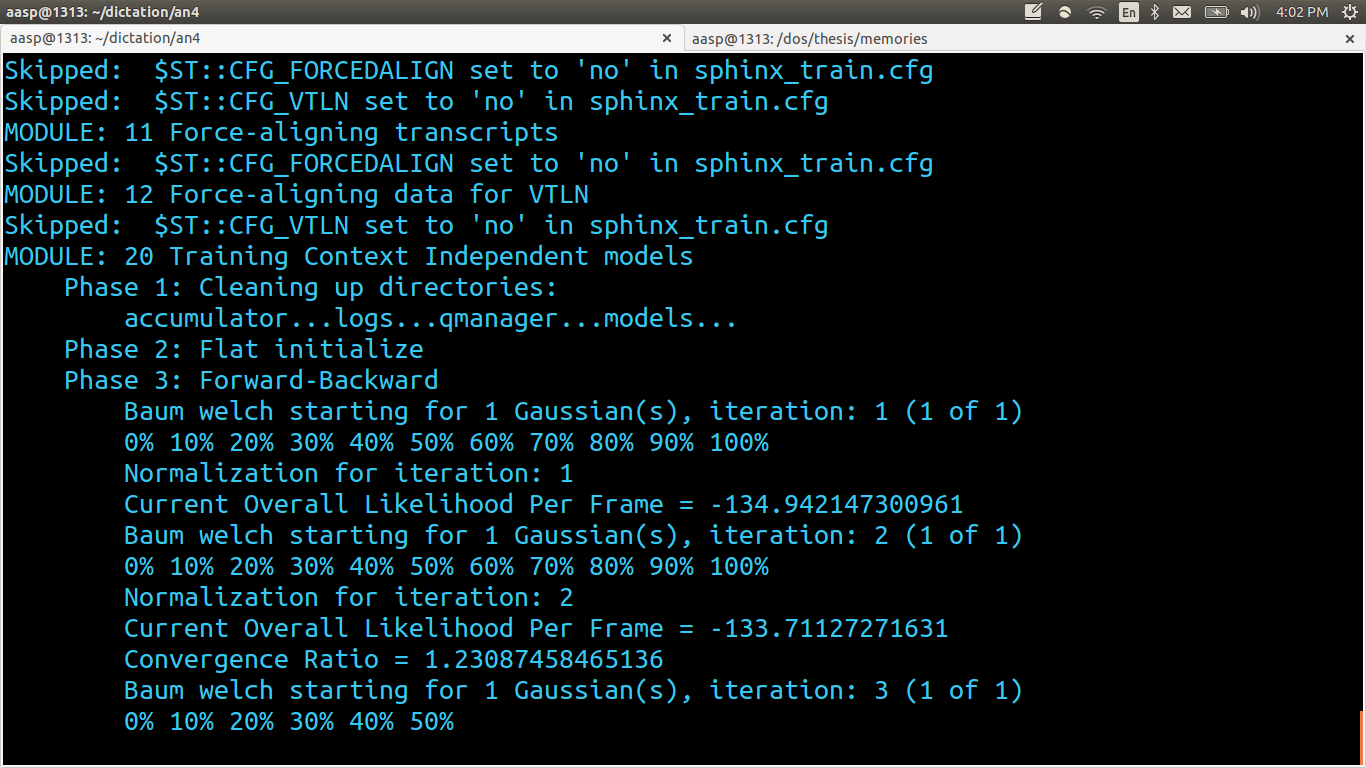
\includegraphics[scale=0.3]{Screenshot3}
    \caption{Training Model}
%    \label{fig:mesh1}
\end{figure}

\subsubsection{Training Internals}
This section describes what happens during the training. In the scripts directory (./scripts\_pl), there are several directories numbered sequentially from 00 through 99. Each directory either has a directory named slave*.pl or it has a single file with extension .pl. The script sequentially goes through the directories and executes either the the slave*.pl or the single .pl file, as below. \\
\textit{
perl scripts\_pl/000.comp\_feat/slave\_feat.pl\\
perl scripts\_pl/00.verify/verify\_all.pl\\
perl scripts\_pl/10.vector\_quantize/slave.VQ.pl\\
perl scripts\_pl/20.ci\_hmm/slave\_convg.pl\\
perl scripts\_pl/30.cd\_hmm\_untied/slave\_convg.pl\\
perl scripts\_pl/40.buildtrees/slave.treebuilder.pl\\
perl scripts\_pl/45.prunetree/slave-state-tying.pl\\
perl scripts\_pl/50.cd\_hmm\_tied/slave\_convg.pl\\
perl scripts\_pl/90.deleted\_interpolation/deleted\_interpolation.pl\\
}


 Scripts launch jobs on your machine, and the jobs will take a few minutes each to run through.

Before you run any script, note the directory contents of your current directory. After you run each slave*.pl note the contents again. Several new directories will have been created. These directories contain files which are being generated in the course of your training. At this point you need not know about the contents of these directories, though some of the directory names may be self explanatory and you may explore them if you are curious.

One of the files that appears in your current directory is an .html file, named model.html, depending on which database you are using. This file will contain a status report of jobs already executed. Verify that the job you launched completed successfully. Only then launch the next slave*.pl in the specified sequence. Repeat this process until you have run the slave*.pl in all directories.

Note that in the process of going through the scripts in 00* through 90*, you will have generated several sets of acoustic models, each of which could be used for recognition. Notice also that some of the steps are required only for the creation of semi-continuous models. If you execute these steps while creating continuous models, the scripts will benignly do nothing. 

 On the stage 000.comp\_feat the feature feles are extracted. The system does not directly work with acoustic signals. The signals are first transformed into a sequence of feature vectors, which are used in place of the actual acoustic signals.

This script slave\_feat.pl will compute, for each training utterance, a sequence of 13-dimensional vectors (feature vectors) consisting of the Mel-frequency cepstral coefficients (MFCCs). Note that the list of wave files contains a list with the full paths to the audio files. Since the data are all located in the same directory as you are working, the paths are relative, not absolute. You may have to change this, as well as the model\_test.fileids file, if the location of data is different. The MFCCs will be placed automatically in a directory called 'feat'. Note that the type of features vectors you compute from the speech signals for training and recognition, outside of this tutorial, is not restricted to MFCCs. You could use any reasonable parameterization technique instead, and compute features other than MFCCs. CMUSphinx can use features of any type or dimensionality. The format of the features is described on the page MFC Format . 

\subsubsection{Testing}
 It's critical to test the quality of the trained database in order to select best parameters, understand how application performs and optimize performance. To do that, a test decoding step is needed. The decoding is now a last stage of the training process.

You can restart decoding with the following command: 
\textit{sphinxtrain -s decode run}
 This command will start a decoding process using the acoustic model you trained and the language model you configured in the \textit{etc/sphinx\_train.cfg} file.

\begin{figure}[h]
    \centering
    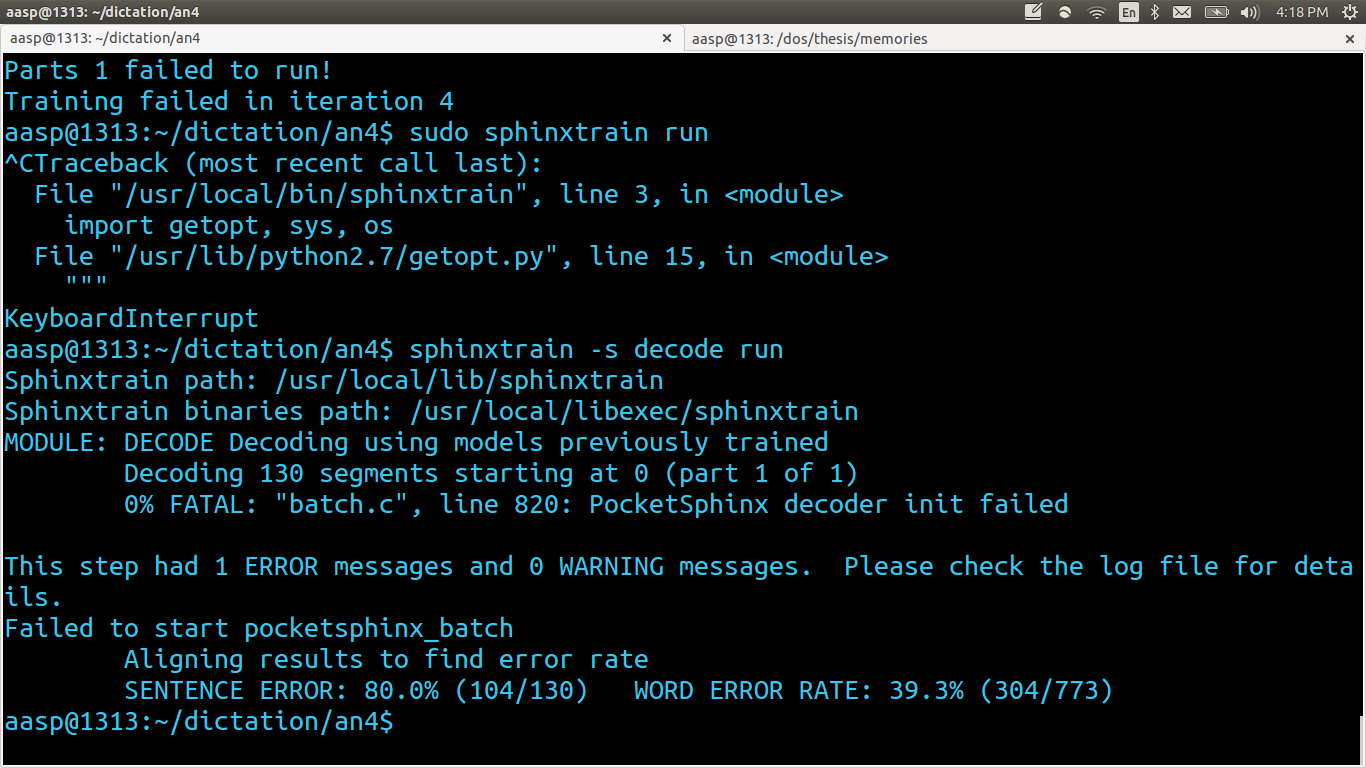
\includegraphics[scale=0.3]{Screenshot4}
    \caption{Testing Model}
%    \label{fig:mesh1}
\end{figure}

\subsubsection{Using the Model}
After training, the acoustic model is located in \\

\textit{model\_parameters/<your\_db\_name>.cd\_cont\_<number\_of senones>}

or in 

\textit{model\_parameters/<your\_db\_name>.cd\_semi\_<number\_of senones>}

The model should have the following files:
\begin{itemize}
	\item[$\bullet$] mdef
	\item[$\bullet$] feat.params
	\item[$\bullet$]mixture\_weights
	\item[$\bullet$]means
	\item[$\bullet$]noisedict
	\item[$\bullet$]transition\_matrices
	\item[$\bullet$]variances
\end{itemize}

Depending on the type of the model you trained. To use the model in pocketsphinx, simply point to it with the -hmm option: \\\\

\textit{pocketsphinx\_continuous -hmm <model\_folder> -lm <some\_lm> -dict <some\_dict>.}

\subsubsection{Output}

The output the model trained for Punjabi language is given in the figure below:



\begin{figure}[h]
    \centering
    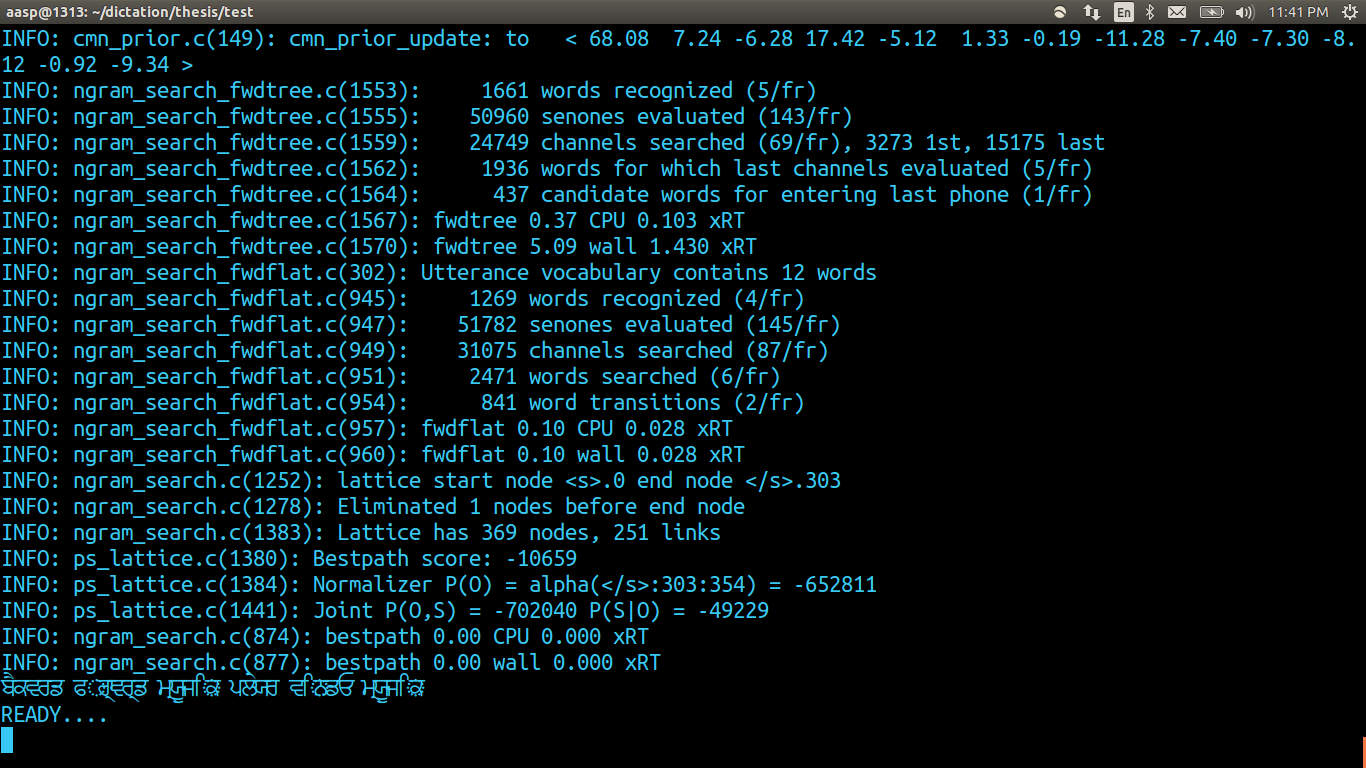
\includegraphics[scale=0.3]{Screenshot5}
    \caption{Punjabi Dictation}
%    \label{fig:mesh1}
\end{figure}

\begin{figure}[h]
    \centering
    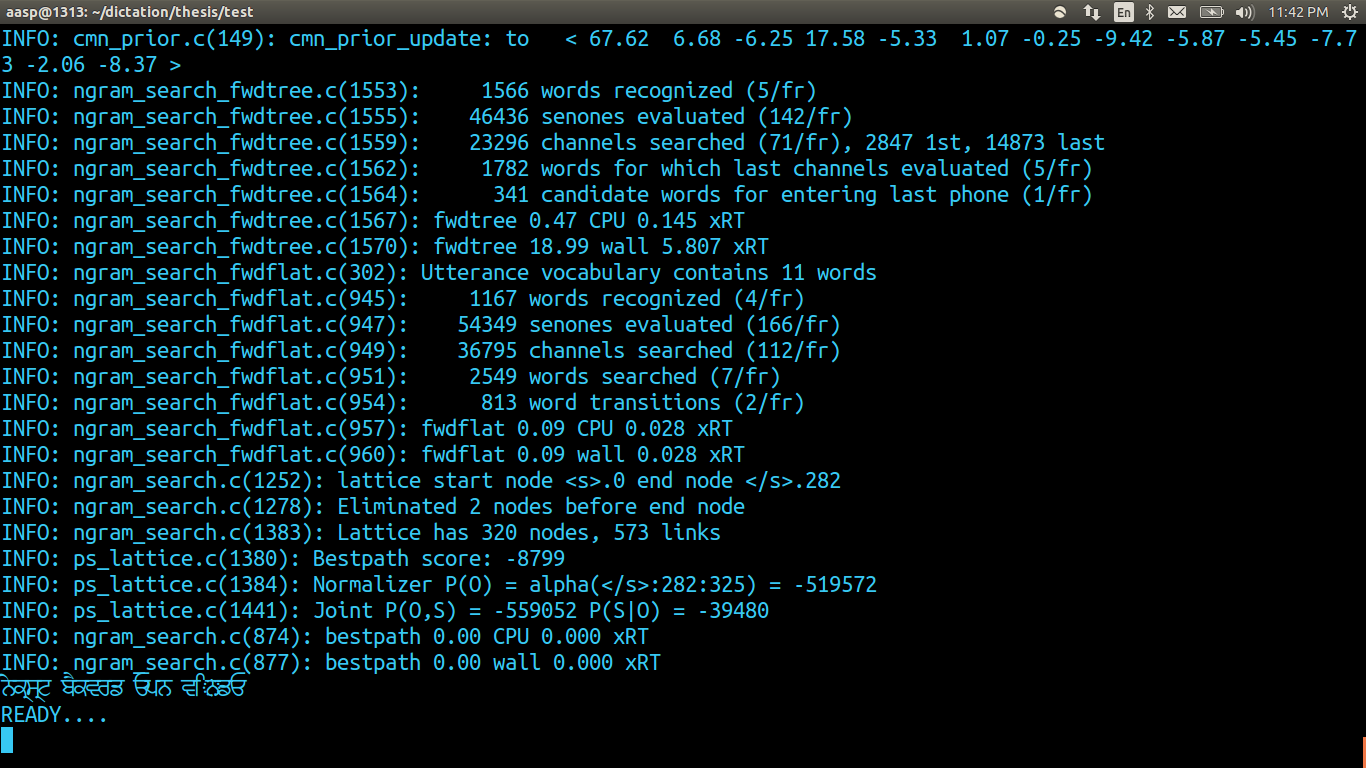
\includegraphics[scale=0.3]{Screenshot6}
    \caption{punjabi Dictation}
%    \label{fig:mesh1}
\end{figure}


%=====================================================================================================================================================
\chapter{CONCLUSION}

\section{Conclusion}
For the past many years, several mechanisms for the communication among human-
machine have been explored. There is much evidence that human speech dictation in
machine involves the integration of a great variety of knowledge sources, including
knowledge of the world or context, knowledge of the speaker and/or topic and many
more. Although there have been significant recent gains in speech dictation, current
technology is far from human-like: only systems in limited domains can be envisioned
in the near term, and the portability of existing techniques is still rather limited.
Application areas that appear to be a good match to technology on the near horizon
include those that are naturally limited.

The objective of the thesis was “speech pattern recognition for speech to text
conversion”. The researcher desire was to pronounced the Punjabi character from any
user, identify it and print it in the text editor. In other word, the recognition of the
Punjabi character or one can say the dictation of the Punjabi character.

\section{Future Work}

The speech dictation is a very huge research work area and required a team of skilled
researcher. Although, the researcher has tried his level best to detect the Punjabi
character. When the idea of the speech dictation was born in the mind of the
researcher, his dream was to dictate the Punjabi continuous speech. The work is of
considerable domain and hence the beginning to end of the work has made with the
detection of Punjabi characters and with its total analysis. So the present study has scope for the
continuation of research for all the remaining Punjabi characters, which further can
be extended in the Punjabi word dictation and ultimately the dictation of words can
again be extended for the continuous speech dictation in Punjabi language.

Although many recent advances and successes in speaker recognition have been
achieved, there are still many possible enhancement for which good solutions are to
be found. Most of these problems arise from variability, including speaker-generated
variability and variability in channel and recording conditions. It is very important to
investigate feature parameters that are stable over time, insensitive to the variation of
speaking manner, including the speaking rate and level, and robust against variations
in voice quality due to causes such as voice disguise or colds and many more ...









%%%%%%%%%%%%%%%%%%%%%%%%%%%%%%%%%%%%%%%%%%%%%%%%%%%%%%%%%%%%%%%%%%%%%%%%%%%%%%%%%%%%%%%%%%%%%%%%%%%%%%%%%%%%%%%%%%%%%%%%%%%%%%%%%%%%%%%%%%%%%%%%%%


%\appendix

%\chapter{Additional}
%Lorem ipsum dolor sit amet, consectetur adipiscing elit, sed do eiusmod tempor incididunt ut labore et dolore magna aliqua. Ut enim ad minim veniam, quis nostrud exercitation ullamco laboris nisi ut aliquip ex ea commodo consequat. Duis aute irure dolor in reprehenderit in voluptate velit esse cillum dolore eu fugiat nulla pariatur. Excepteur sint occaecat cupidatat non proident, sunt in culpa qui officia deserunt mollit anim id est laborum.
%%%%%%%%%%%%%%%%%%%%%%%%%%%%%%%%%%%%%%%%%%%%%%%%%%%%%%%%%%%%%%%%%%%%%%%%%%%%%%%%%%%%%%%%%%%%%%%%%%%%%%%%%%%%%%%%%%%%%%%%%%%%%%%%%%%%%%%%%%%%%%%%%%


%=====================================================================================================================================================


%\bibliographystyle{unsrt}
%\bibliography{sample}

%\printbibliography[title=References]


\begin{thebibliography}{9}

\bibitem{1}
Chowdhury, Gobinda G. 
"Natural language processing."
%Annual review of information science and technology 37.1 (2003): 51­89.
\textit{Annual review of information science and technology 37.1,} 2003: 5189.

\bibitem{2}
Kaur, Navdeep,Vandana Pushe, and Rupinderdeep Kaur.
Natural Language Processing Interface for Synonym."
\textit{from outside the contents of the document,} 2014.

\bibitem{3}
Kaur, Kamaldeep, and Vishal Gupta.
"Name and Entity Recognition for Punjabi Language."
\textit{Machine translation 2.3,} 2012.

\bibitem{4}Necula, George C."Translation validation for an optimizing compiler."
\textit{ACM sigplan notices. Vol. 35. No. 5. ACM,} 2000.


\bibitem{5}Mac, David, Tom, and Alexendre. "GNU Automake."
\textit{User Manual, for Automake version 1,} 1995.

\bibitem{6} Calcote, John. "Autotools: A Practitioner's"
\textit{Guide to GNU Autoconf, Automake, and Libtool. No Starch Press,} 2010.

\bibitem{7}Byrne, William, et al. "Towards language independent acoustic modeling."
\textit{Acoustics, Speech, and Signal Processing,} 2000. ICASSP'00. Proceedings. 2000 IEEE International Conference on. Vol. 2. IEEE, 2000.

\bibitem{8}Lippmann, Richard P. "Speech recognition by machines and humans."
\textit{Speech communication 22.1,} 1997.

\bibitem{9} Schultz, TAnja, and Alex. "Language independent and languge adaptive acoustic model for speech recognition."
\textit{Speech Communication 35.1,} 2001.

\bibitem{10} Walker, Willie, et al. "Sphinx4: A flexible open source framework for speech recognition,", 2004.
\textit{}

\bibitem{11}Sankar, Fuliang Weng Andreas Stolcke Ananth. "Efficient Lattice Representation and Generation.", 2006.
\textit{}

\bibitem{12} Dua, Mohit, et al. "Punjabi automatic speech recognition using HTK."
\textit{IJCSI International Journal of Computer Science Issues 9.4,} 2012.


\bibitem{13} Ravinder, Kumar. "Comparison of hmm and dtw for isolated word recognition system of punjabi language."
\textit{Progress in Pattern Recognition, Image Analysis, Computer Vision, and Applications. Springer Brelin,} 2010.

\bibitem{14}Grasch, Peter, Alexander Felfernig, and Florian Reinfrank. "ReComment: Towards critiquing-
based recommendation with speech interaction."
\textit{Proceedings of the 7th ACM Conference on Recommender Systems. ACM,} 2013.

\bibitem{15}Ravinder, and Rajendra Kumar Sharma. "An efficient post processing algorithm for online handwriting Gurmukhi character recognition using set theory."
\textit{International Journal of Pattern Recognition and Artificial Intelligence 27.04,} 2013.

\bibitem{16}Bansal, Divya, Ankita Goel, and Khushneet Jindal. "Punjabi Speech Synthesis System Using Htk."
\textit{International Journal of Information 2.4,} 2012.

\bibitem{17}Dua, Mohit, et al. "Punjabi speech to text system for connected words.", 2012.
\textit{}

\bibitem{18}Ghai, Wiqas, and Navdeep Singh. "Continuous Speech Recognition for Punjabi."2013.
\textit{}

\bibitem{19}
http://www.programmershare.com/
%\textit{}

\bibitem{20}
http://cmusphinx.sourceforge.net/wiki/
%\textit{}

\bibitem{21}
[6]Kumbharana, Chandresh K."Speech Pattern Recognition for Speech to Text Conversion."
\textit{Diss. Saurashtra University,} 2007.

\bibitem{22} Electronics for U may 2000
%\textit{}

\bibitem{23}IBM, Developing voice applications.
%\textit{}

\bibitem{24} https://en.wikipedia.org/wiki/Ubuntu\_(28operating\_system)
\textit{}

\bibitem{25}http://www.gnu.org/software/bison/
\textit{}

\bibitem{26}http://www.swig.org/Doc1.3/Library.html
\textit{}

\bibitem{27}https://en.wikipedia.org/wiki/GStreamer
\textit{}

\bibitem{28}http://gstreamer.freedesktop.org/features/
\textit{}

\bibitem{29}https://launchpad.net/ubuntu/precise/+package/pythondev
\textit{}

\bibitem{30}http://sourceforge.net/projects/cmusphinx/files/sphinxtrain/5prealpha/
\textit{}

\bibitem{31}https://www.gnu.org/software/automake/
\textit{}



\end{thebibliography}




\end{document}

\grid
